\documentclass[11pt,a4paper]{article}

\usepackage[margin=2.05cm]{geometry}
\usepackage[T1]{fontenc}
\usepackage[utf8]{inputenc}
\usepackage{lmodern}
\usepackage{microtype}
\usepackage{booktabs}
\usepackage{tabularx}
\usepackage{array}
\usepackage{enumitem}
\usepackage{xcolor}
\usepackage{hyperref}
\usepackage{graphicx}
\usepackage{float}

\graphicspath{{../assets/}}
\hypersetup{
  colorlinks=true,
  linkcolor=blue,
  urlcolor=blue,
  citecolor=blue,
  hypertexnames=false
}

\setlist[itemize]{leftmargin=1.35em,itemsep=0.15em,topsep=0.2em}
\setlist[enumerate]{leftmargin=1.45em,itemsep=0.15em,topsep=0.2em}
\renewcommand{\arraystretch}{1.15}
\setlength{\parindent}{0pt}
\setlength{\parskip}{0.45em}
\emergencystretch=3em
\newcommand{\code}[1]{\texttt{\detokenize{#1}}}

\title{\vspace{-1.0cm}CyberSecIntel\\P2 Follow-Up Deliverable 2.2\\Basic Implementation}
\author{D\'idac Cayuela and Sindri Masson\\Big Data Management -- Universitat Politecnica de Catalunya}
\date{May 2026}

\begin{document}

\maketitle
\vspace{-0.7cm}

\section{Instructions}

This follow-up implements the basic data movement required by P2. The objective is not to finalize every transformation, but to prove that the architecture from Deliverable 2.1 is executable end to end: P1 landing/silver Delta tables are read, Trusted Zone checkpoints are written, Exploitation Zone assets are materialized, and consumption files are exported for analysts.

The implementation uses the same Option 1 architecture selected in P2.1. MinIO and Delta Lake remain the source of truth for all zones. The new buckets are \code{s3://trusted/} and \code{s3://exploitation/}; the original P1 Delta bucket \code{s3://deltalake/} is unchanged.

\textbf{Run order.}
\begin{enumerate}
  \item Start the stack: \code{docker compose up -d minio zookeeper kafka postgres}, then initialize and start Airflow.
  \item Run the P1 ingestion DAGs: \code{cybersecintel\_api\_expansion\_ingestion}; optionally run \code{cybersecintel\_dataset\_artifact\_ingestion} and \code{cybersecintel\_pcap\_replay}.
  \item Trigger \code{cybersecintel\_trusted\_zone}.
  \item Trigger \code{cybersecintel\_exploitation\_zone}.
  \item Trigger \code{cybersecintel\_consumption\_exports}.
\end{enumerate}

The same stages can be run without Airflow:
\begin{verbatim}
python -m trusted.run_trusted
python -m exploitation.run_exploitation --warm
python -m consumption.run_exports
\end{verbatim}

\section{Architecture Design}

\begin{figure}[H]
  \centering
  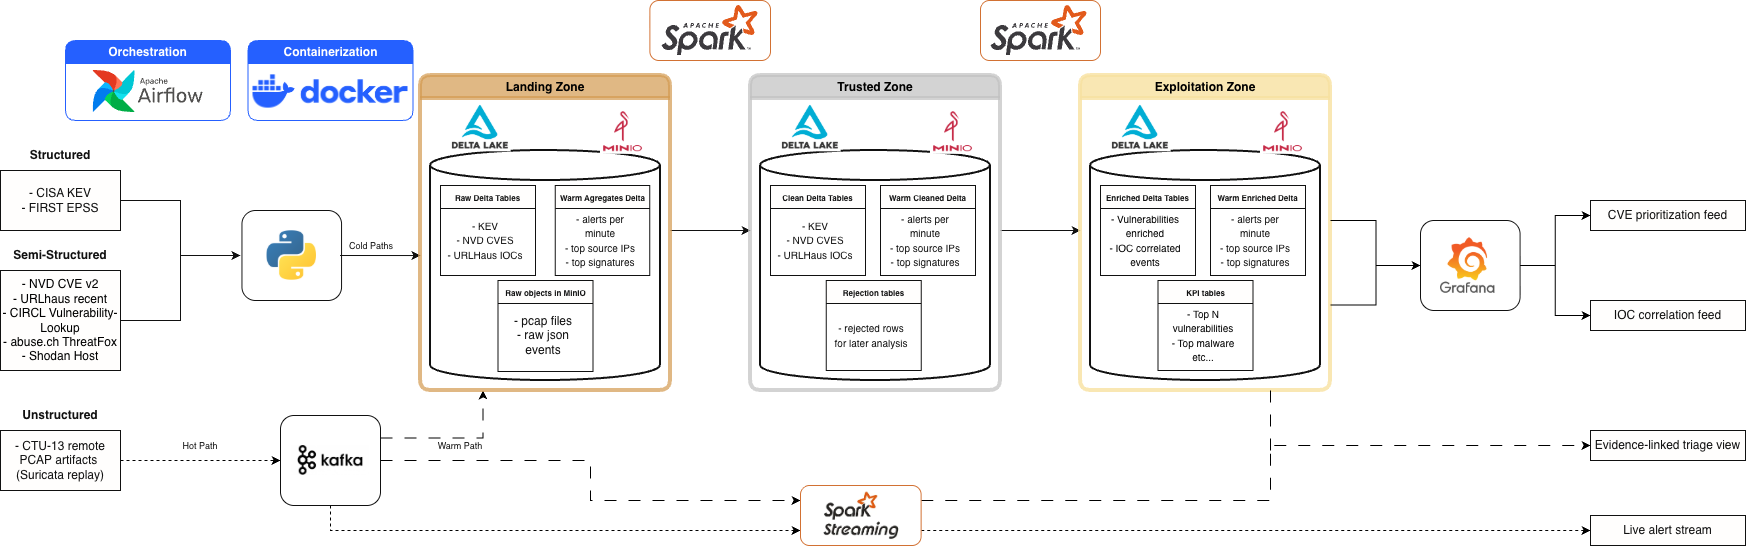
\includegraphics[width=\textwidth,height=0.58\textheight,keepaspectratio]{BDM_P2.drawio.png}
  \caption{P2 architecture implemented in this follow-up. P2.2 focuses on executable zone checkpoints and basic consumption outputs.}
\end{figure}

\begin{tabularx}{\textwidth}{>{\raggedright\arraybackslash}p{3.2cm}X}
\toprule
\textbf{Component} & \textbf{P2.2 implementation}\\
\midrule
Trusted Zone & Top-level \code{trusted/} package. Reads existing P1 Delta tables from \code{s3://deltalake/}, performs conservative cleaning, and writes cleaned and rejected rows to \code{s3://trusted/}.\\
Exploitation Zone & Top-level \code{exploitation/} package. Reads trusted tables and writes \code{vuln\_enriched}, \code{network\_events}, \code{ioc\_correlations}, \code{anomaly\_flags}, \code{warm\_enriched\_alerts}, and KPI tables to \code{s3://exploitation/}.\\
Consumption & Top-level \code{consumption/} package. Exports CSV, JSON, and HTML analyst artifacts under \code{consumption/outputs/}.\\
Orchestration & Three new Airflow DAGs: \code{cybersecintel\_trusted\_zone}, \code{cybersecintel\_exploitation\_zone}, and \code{cybersecintel\_consumption\_exports}.\\
Streaming & A bounded warm-path consumer reads a finite batch from Kafka topic \code{ids.alerts}, enriches alerts when CVE context is available, and writes \code{warm\_enriched\_alerts}.\\
\bottomrule
\end{tabularx}

\section{Trusted Zone}

The Trusted Zone applies information-preserving cleaning. The code does not remove analytical signals or perform task-specific modeling. It standardizes key fields, casts common numeric fields, normalizes CVE identifiers, validates basic dates and URLs, deduplicates by natural keys, and records quality warnings.

Rows that fail mandatory-field checks are written to \code{rejected\_*} tables. Duplicate rows are also preserved there with a rejection reason. This keeps the cleaning stage auditable while giving downstream tasks a cleaner checkpoint.

\begin{tabularx}{\textwidth}{>{\raggedright\arraybackslash}p{3.2cm}X}
\toprule
\textbf{Source family} & \textbf{Basic trusted implementation}\\
\midrule
Structured & \code{kev} and \code{epss}: CVE normalization, mandatory-field checks, deduplication, date parsing, EPSS range warnings.\\
Semi-structured & \code{nvd}, \code{urlhaus}, \code{circl\_vulnlookup}, \code{threatfox}, and \code{shodan\_seeded}: stable helper fields, CVE or indicator normalization, basic URL and score warnings.\\
Network / unstructured-derived & \code{pcap\_artifacts}, \code{pcap\_replay\_runs}, \code{suricata\_events}, and \code{ids\_alerts}: timestamp validation, integer casting, deduplication, and ingest-date preservation.\\
\bottomrule
\end{tabularx}

\section{Exploitation Zone}

The Exploitation Zone materializes analyst-ready assets:
\begin{itemize}
  \item \code{vuln\_enriched}: CVE-level table joining KEV, NVD, EPSS, and CIRCL by normalized CVE id.
  \item \code{network\_events}: unified schema for trusted IDS alerts and Suricata events.
  \item \code{ioc\_correlations}: matches URLhaus, ThreatFox, and Shodan indicators against observed network fields when possible.
  \item \code{anomaly\_flags}: rule-based P2.2 anomaly feed using severity, repeated source IPs, and suspicious destination ports.
  \item KPI tables: top CVEs by priority, daily alert counts, top signatures, top source IPs, and recent KEV additions.
\end{itemize}

The vulnerability priority score follows the P2.1 idea: combine EPSS likelihood, KEV active exploitation evidence, and CVSS severity when present. If CVSS is unavailable in the current P1 source snapshot, the score still remains usable through EPSS and KEV.

\section{Data Consumption}

The consumption stage writes concrete files under \code{consumption/outputs/}:
\begin{itemize}
  \item \code{cve\_prioritization.csv}
  \item \code{ioc\_correlations.csv}
  \item \code{anomaly\_flags.csv}
  \item \code{alert\_trends.json}
  \item \code{soc\_dashboard.html}
\end{itemize}

Grafana is intentionally not introduced in this checkpoint. The current deliverable proves the data contracts and visible outputs first. A Grafana service can be added in the final P2 phase by mirroring selected KPI tables into a serving database while keeping Delta Lake as the authoritative source.

\section{What Remains for Final P2}

The final delivery should improve transformation depth and governance. The main remaining work is richer source-specific cleaning, stronger schema documentation, a more complete lineage table, optional Grafana provisioning, and replacing the rule-based anomaly feed with the Isolation Forest model proposed in P2.1 if time permits.

\section{Validation}

The implementation includes unit tests for trusted cleaning, exploitation joins and KPIs, warm-path enrichment, and consumption exports. Run:
\begin{verbatim}
.venv/bin/python -m unittest discover -s tests
\end{verbatim}

For integration validation, inspect MinIO after running the DAGs and confirm that the \code{trusted} and \code{exploitation} buckets exist. Then open \code{consumption/outputs/soc\_dashboard.html} and verify that the generated CSV/JSON files exist.

\end{document}
